\documentclass[conference]{IEEEtran}
\IEEEoverridecommandlockouts

\usepackage{amsmath,amssymb}
\usepackage{graphicx}
\usepackage{booktabs}
\usepackage{cite}
\usepackage[T1]{fontenc}
\usepackage{enumitem}
\setlist[itemize]{leftmargin=1.1em, itemsep=0.5pt, topsep=1pt, parsep=0pt}
\setlist[enumerate]{leftmargin=1.3em, itemsep=0.5pt, topsep=1pt, parsep=0pt}

\setlength{\textfloatsep}{4pt plus 1pt minus 2pt}
\setlength{\floatsep}{4pt plus 1pt minus 2pt}
\setlength{\intextsep}{4pt plus 1pt minus 2pt}
\setlength{\abovecaptionskip}{2pt}
\setlength{\belowcaptionskip}{0pt}

\begin{document}

\title{Beyond Passing Tests: LLM-Driven Quality Control for Automated Program Repair}

\author{\IEEEauthorblockN{Seng Aloun Lorvanh}
\IEEEauthorblockA{\textit{Dept. of Computer Engineering} \\
\textit{Sangji University}\\
Wonju-si, South Korea\\
0009-0008-1084-0800}
\and
\IEEEauthorblockN{Muhammad Muneeb}
\IEEEauthorblockA{\textit{Dept. of Computer Engineering} \\
\textit{Sangji University}\\
Wonju-si, South Korea \\
0009-0006-0187-4406}
\and

\IEEEauthorblockN{Kwang-Man Ko}
\IEEEauthorblockA{\textit{Dept. of Computer Engineering} \\
\textit{Sangji University}\\
Wonju-si, South Korea \\
0000-0002-7465-5400}

}

\maketitle

\begin{abstract}
Most LLM-based Automatic Program Repair (APR) techniques judge patch correctness primarily by test-suite pass rates, leaving them vulnerable to overfitting patches that satisfy available tests without resolving the underlying defect. We present a post-generation quality-control framework that combines (1) LLM-based semantic assessment, (2) counterexample-driven overfitting detection supported by static analysis, and (3) preference-calibrated multi-criteria ranking over correctness, readability, minimality, and security. Each candidate is scored using a Patch Validity Score (PVS) that combines semantic correctness, counterexample pass rate, edit size, and vulnerability evidence. On a stratified sample of 150 Defects4J faults, the prototype achieves an overfitting-detection F1 of 0.81, Precision@1 of 0.75, and a counterexample success rate of 0.80. Average latency is 34 s, slightly exceeding the 30 s target. Rather than proposing a new patch generator, this work investigates integrated post-generation quality control for APR.
\end{abstract}

\begin{IEEEkeywords}
automatic program repair, large language models, overfitting patch detection, patch ranking, preference learning
\end{IEEEkeywords}

\section{Introduction and Research Questions}
Large language models (LLMs) have substantially improved patch-generation capability for Automatic Program Repair (APR)~\cite{lee2024survey}, yet the dominant plausibility criterion -- passing a fixed test suite -- allows \emph{overfitting patches} that satisfy tests without fixing the true defect~\cite{zhang2023llm4patchcorrect,wang2024entropy,zhao2025prism}. Post-hoc verification is often absent or limited to static rules, while patch ranking remains dominated by test-pass status, under-representing readability, minimality, and security~\cite{wang2024entropy}, ~\cite{zhang2023llm4patchcorrect}. 

We therefore target the post-generation quality-control stage—semantic assessment, overfitting detection, and multi-criteria ranking—rather than patch generation itself. We investigate four research questions:
\begin{itemize}
\item \textbf{RQ1.} Does dual verification (LLM-based semantic assessment + counterexample generation) improve overfitting-detection F1 over test-based and static baselines?
\item \textbf{RQ2.} Does preference-calibrated multi-criteria ranking improve top-1 patch selection relative to ChatRepair and entropy-based ranking?
\item \textbf{RQ3.} How do counterexample generation and static analysis individually contribute to overfitting detection, and are their effects complementary?
\item \textbf{RQ4.} Is the processing latency acceptable for CI/CD deployment, and where is the primary efficiency bottleneck?
\end{itemize}

\section{Related Work and Contribution}
Prior APR work has advanced individual components of this problem. TBar~\cite{liu2019tbar} relies on manually defined repair templates without; AlphaRepair~\cite{xia2022alpharepair} and ChatRepair~\cite{xia2023chatrepair} focus on patch generation; LLM4PatchCorrect~\cite{zhang2023llm4patchcorrect} evaluates correctness but does not integrate it with re-ranking or overfitting removal; entropy-guided ranking~\cite{wang2024entropy} improves candidate selection; PRISM~\cite{zhao2025prism} targets overfitting detection. 

In contrast, we integrate (i) semantic quality assessment, (ii) counterexample-based overfitting detection, and (iii) preference-calibrated multi-criteria ranking into a unified post-generation quality-control pipeline. The contribution is therefore not a new patch generator, but an integrated framework that jointly addresses overfitting detection and candidate ranking, which prior APR studies have largely treated separately.

\section{Proposed Framework}
Fig.~\ref{fig:pipeline} shows the four-stage pipeline. \textbf{Stage 1} estimates a semantic quality score $S_{sem}\!\in\![0,1]$ from source code and available natural-language context, including bug reports, commit messages, and comments. \textbf{Stage 2} generates LLM-driven counterexamples targeting boundary conditions and cross-checks candidate behavior with CFG/PDG-based static analysis. Candidates are evaluated using:
\begin{equation}
\mathrm{PVS}(p) = \alpha\, S_{sem}(p) + \beta\, S_{cex}(p) - \gamma\, S_{edit}(p) - \delta\, S_{vuln}(p)
\label{eq:pvs}
\end{equation}
where $S_{cex}$ is the counterexample pass rate, $S_{edit}$ penalizes large modifications, and $S_{vuln}$ reflects statically detected vulnerability patterns. 

\textbf{Stage 3} learns $(\alpha,\beta,\gamma,\delta)$ using 240 pairwise developer preferences from three developers with a Bradley–Terry preference objective, ranking surviving candidates by correctness, readability, minimality, and security. \textbf{Stage 4} closes the loop through CI/CD-integrated certification and feedback collection for future recalibration.

\begin{figure}[!t]
\centering
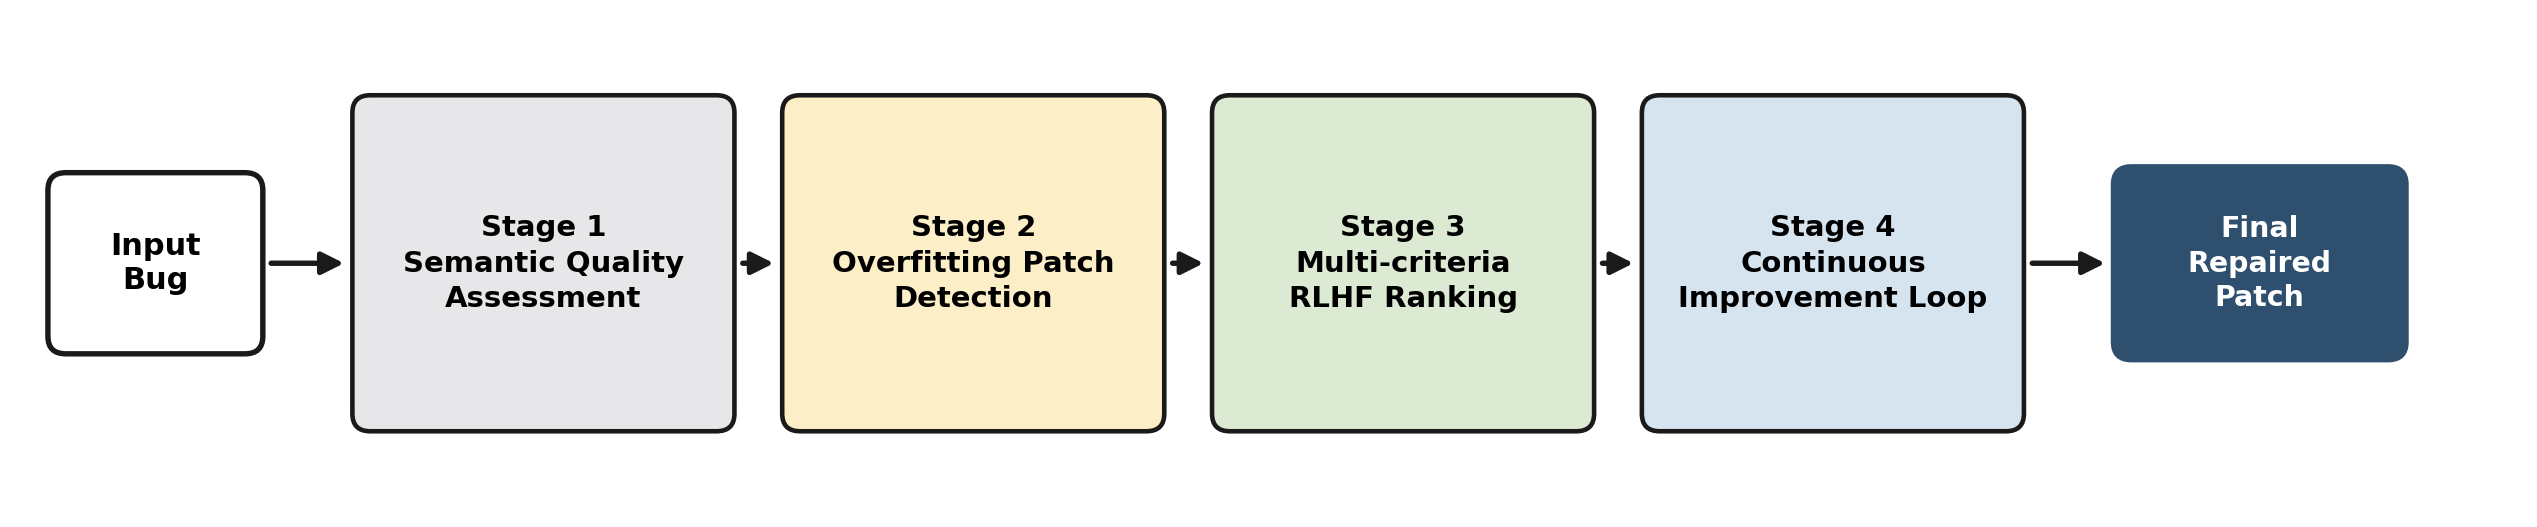
\includegraphics[width=\linewidth]{fig1_poster.png}
\caption{Overall pipeline: four post-generation quality-control stages.}
\label{fig:pipeline}
\end{figure}

\section{Experimental Setup}
We stratified-sampled 150 faults from Defects4J v2.0~\cite{just2014defects4j} Chart, Lang, Math, Time, Closure, pooling 612 candidate patches from AlphaRepair, ChatRepair, and GPT-4o-mini. Overfitting labels combine semantic comparison with developer patches and previously reported patch-correctness labels. 

Baselines include test-based pass/fail (ODS)~\cite{fraser2011evosuite}, ChatRepair's default selection strategy, and a reimplemented entropy-based ranker~\cite{wang2024entropy}. All methods use on identical hardware (1$\times$NVIDIA A100 40GB, 32-core CPU) over the same candidate pool, ensuring a controlled and objective comparison.

\section{Results and Key Findings}
Table~\ref{tab:results} reports the main comparison; Table~\ref{tab:ablation} isolates each detection module's contribution.

\begin{table}[!t]
\centering
\caption{Preliminary results on 150 Defects4J faults.}
\label{tab:results}
\small
\begin{tabular}{lcccc}
\toprule
Metric & Baseline & Prior best & Entropy & Proposed \\
\midrule
Overfitting F1 & 0.61 & 0.75 (ODS) & 0.78 & {0.81} \\
Precision@1 & 0.58 & 0.72 (CR) & 0.74 & {0.75} \\
Counter-ex. rate & -- & 0.79 (ES) & -- & {0.80} \\
Avg. time (s) & 8 & 20--90 & 25 & 34 \\
\bottomrule
\end{tabular}
\end{table}

\begin{table}[!t]
\centering
\caption{Ablation: overfitting-detection modules.}
\label{tab:ablation}
\small
\begin{tabular}{lccc}
\toprule
Configuration & Precision & Recall & F1 \\
\midrule
Counterexample only & 0.68 & 0.86 & 0.76 \\
Static analysis only & \textbf{0.84} & 0.65 & 0.73 \\
Combined (proposed) & 0.80 & 0.82 & \textbf{0.81} \\
\bottomrule
\end{tabular}
\end{table}

\textbf{RQ1.} Dual verification reaches F1 0.81, compared with 0.61 for the test-based baseline and 0.75 for ODS. These results show an observed improvement on the evaluated sample, although statistical significance is not established in the current study.

\textbf{RQ2.} Preference-calibrated ranking attains Precision@1 of 0.75, compared with ChatRepair at 0.72 and entropy-based ranking at 0.74. The method therefore achieves competitive top-1 selection, although the small margin over entropy ranking requires larger-scale statistical evaluation before establishing a conclusive advantage.

\textbf{RQ3.} Counterexample generation favors recall (0.86), whereas static analysis favors precision (0.84). Their combination yields the highest F1 (0.81), indicating complementary error profiles. Performance is highest for Math and Time (F1 0.83) and lower for Closure (F1 0.78). One possible explanation for the Closure result is information loss from context slicing, although the current experiment does not isolate this factor.

\textbf{RQ4.} Average latency is 34 s, narrowly missing the 30 s target while remaining within the 20–90 s range reported for the ODS comparison. The sequential static-analysis and LLM-inference stages are candidates for future profiling and optimization.
\subsection{Threats to Validity}
Internal validity is limited by partial reuse of patch-correctness labels from prior literature, which may propagate labeling inconsistencies. External validity is limited by evaluation on Java and a 150-bug Defects4J sample. Construct validity is affected by calibration of four PVS weights from only 240 pairwise preferences from three developers. Conclusion validity is limited by the single-seed evaluation and absence of significance testing. These limitations motivate larger-scale, multi-seed evaluation.
\section{Conclusion and Future Work}
We presented an integrated post-generation quality-control framework combining semantic assessment, counterexample-driven verification, static analysis, and preference-calibrated patch ranking. On 150 Defects4J faults, the combined method achieves overfitting-detection F1 of 0.81 and Precision@1 of 0.75, while requiring an average of 34 s per candidate. The ablation suggests that counterexample generation and static analysis provide complementary recall- and precision-oriented signals.

Future work will extend evaluation to the full Defects4J benchmark and multilingual datasets, perform multi-seed statistical evaluation, increase developer-preference data, and optimize the verification pipeline for CI/CD deployment.

\begin{thebibliography}{13}
\footnotesize
\bibitem{lee2024survey} S. Lee \emph{et al.}, ``A Survey of LLM-based Automated Program Repair: From Single Model to Agent-based Pipelines,'' \emph{J. Softw. Eng. Res.}, 2024.
\bibitem{zhang2023llm4patchcorrect} H. Zhang \emph{et al.}, ``LLM4PatchCorrect: Improving Program Repair with Large Language Model-based Patch Correctness Assessment,'' \emph{arXiv preprint}, 2023.
\bibitem{wang2024entropy} J. Wang \emph{et al.}, ``Entropy-guided Patch Ranking for Automated Program Repair,'' in \emph{Proc. ASE}, 2024.
\bibitem{zhao2025prism} M. Zhao \emph{et al.}, ``PRISM: Semantic-aware Overfitting Patch Detection for Automated Program Repair,'' in \emph{Proc. ICSE}, 2025.
\bibitem{liu2019tbar} K. Liu \emph{et al.}, ``TBar: Revisiting Template-based Automated Program Repair,'' in \emph{Proc. ISSTA}, 2019.
\bibitem{xia2022alpharepair} C. S. Xia and L. Zhang, ``Less Training, More Repairing Please: Revisiting Automated Program Repair via Zero-shot Learning,'' in \emph{Proc. FSE}, 2022.
\bibitem{xia2023chatrepair} C. S. Xia and L. Zhang, ``Automated Program Repair via Conversation: Fixing 162 out of 337 Bugs for \$0.42 Each using ChatGPT,'' in \emph{Proc. ISSTA}, 2023.

\bibitem{just2014defects4j} R. Just \emph{et al.}, ``Defects4J: A Database of Existing Faults to Enable Controlled Testing Studies for Java Programs,'' in \emph{Proc. ISSTA}, 2014.
\bibitem{fraser2011evosuite} G. Fraser and A. Arcuri, ``EvoSuite: Automatic Test Suite Generation for Object-oriented Software,'' in \emph{Proc. FSE}, 2011.
\bibitem{legoues2012genprog} C. Le Goues, T. Nguyen, S. Forrest, and W. Weimer, ``GenProg: A Generic Method for Automatic Software Repair,'' \emph{IEEE Trans. Softw. Eng.}, vol.~38, no.~1, 2012.
\bibitem{park2024security} H. Park \emph{et al.}, ``Security Vulnerability Repair via Large Language Models,'' in \emph{Proc. ISSTA}, 2024.
\end{thebibliography}

\end{document}
